\chapter{Benchmarks}

In this chapter, we measure the performance of our implementation. We quantify the impact of different input size and algorithm parameters. In the end, we compare our implementation with an original python implementation of the algorithm.

All the data was measured using an NVIDIA RTX 3080 graphics card with Intel i5 6600K processor. We used an M.2 SSD disk.

\todo{methodology? Each value presented in this chapter is a mean of several runs of the whole algorithm. Every time, we start the whole computation and measure runs of all kernels and take average from all the runs of kernels within one run of application. We repeat the process several times with the same parameters and take the average, then start over with different set of parameters.}

We measure only square subregions, because it removes unnecessary complexity from the benchmarks. In theory, whole algorithm works also for rectangle--shaped subregions, but since we analyze the direction in which the subregions are shifted, the square should have the same dimensions in each direction.

\section{Relative performance of individual parts}

\begin{figure}
	\centering
	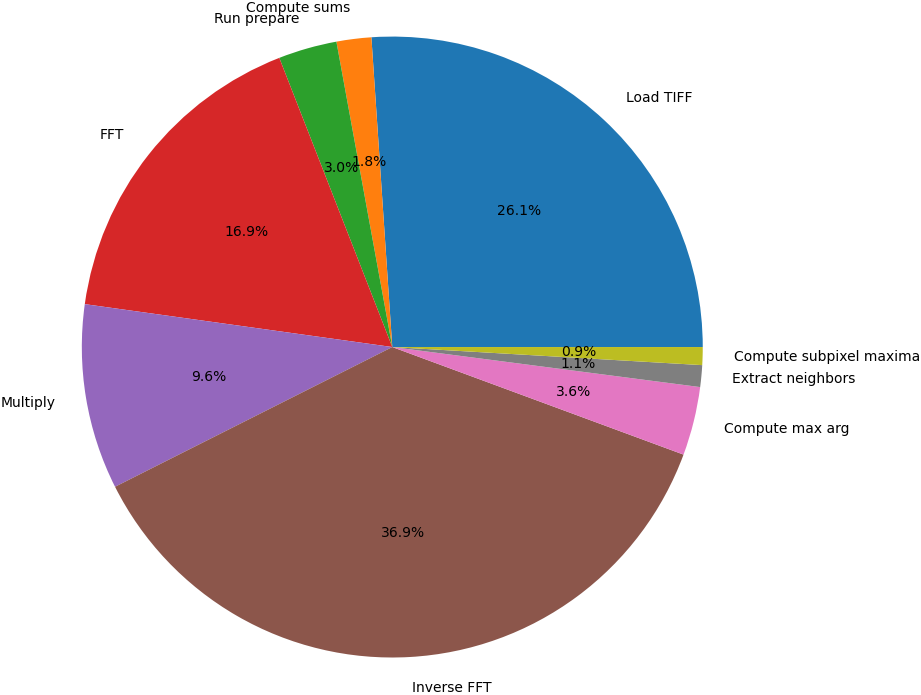
\includegraphics[width=0.7\textwidth]{img/eval/individual-parts}
	\caption{Relative performance of individual parts of the algorithm. The data was measured from a run of the algorithm with a configuration of 90 subregions with size $120 \times 120$. The size of the neigborhood was set to maximal value 9. }
	\label{individual-parts}
\end{figure}

We begin with an overview of all the kernels used in the implementation. \Cref{individual-parts} shows how much time the implementation spends in individual kernels. We can see, that the most demanding parts are loading of the TIFF and the cross--correlation, which is computed using the multiply kernel and the Fourier transforms.

The figure is mentioned here only to get general idea about the performance. It captures relative performance of the kernels for 90 subregions with size $120 \times 120$, which is roughly in the middle of the range of expected values. Different parts depend on different parameters, so for some other input size, the relative performance would look dissimilar. The load TIFF subroutine depends only on the size of the TIFF, while the rest of the algorithm depends on the number of subregion. So, for instance, it is possible to find a configuration that makes load TIFF the longest part. 

\section{Cross--correlation}
First, we measure the performance of cross--correlation when computed using Fourier transform. We show the dependence between running time and size and number of subregions. Since the cross--correlation is computed using three parts, we analyze them one by one.


\subsection{Fourier transforms}
\begin{figure}
	\centering
	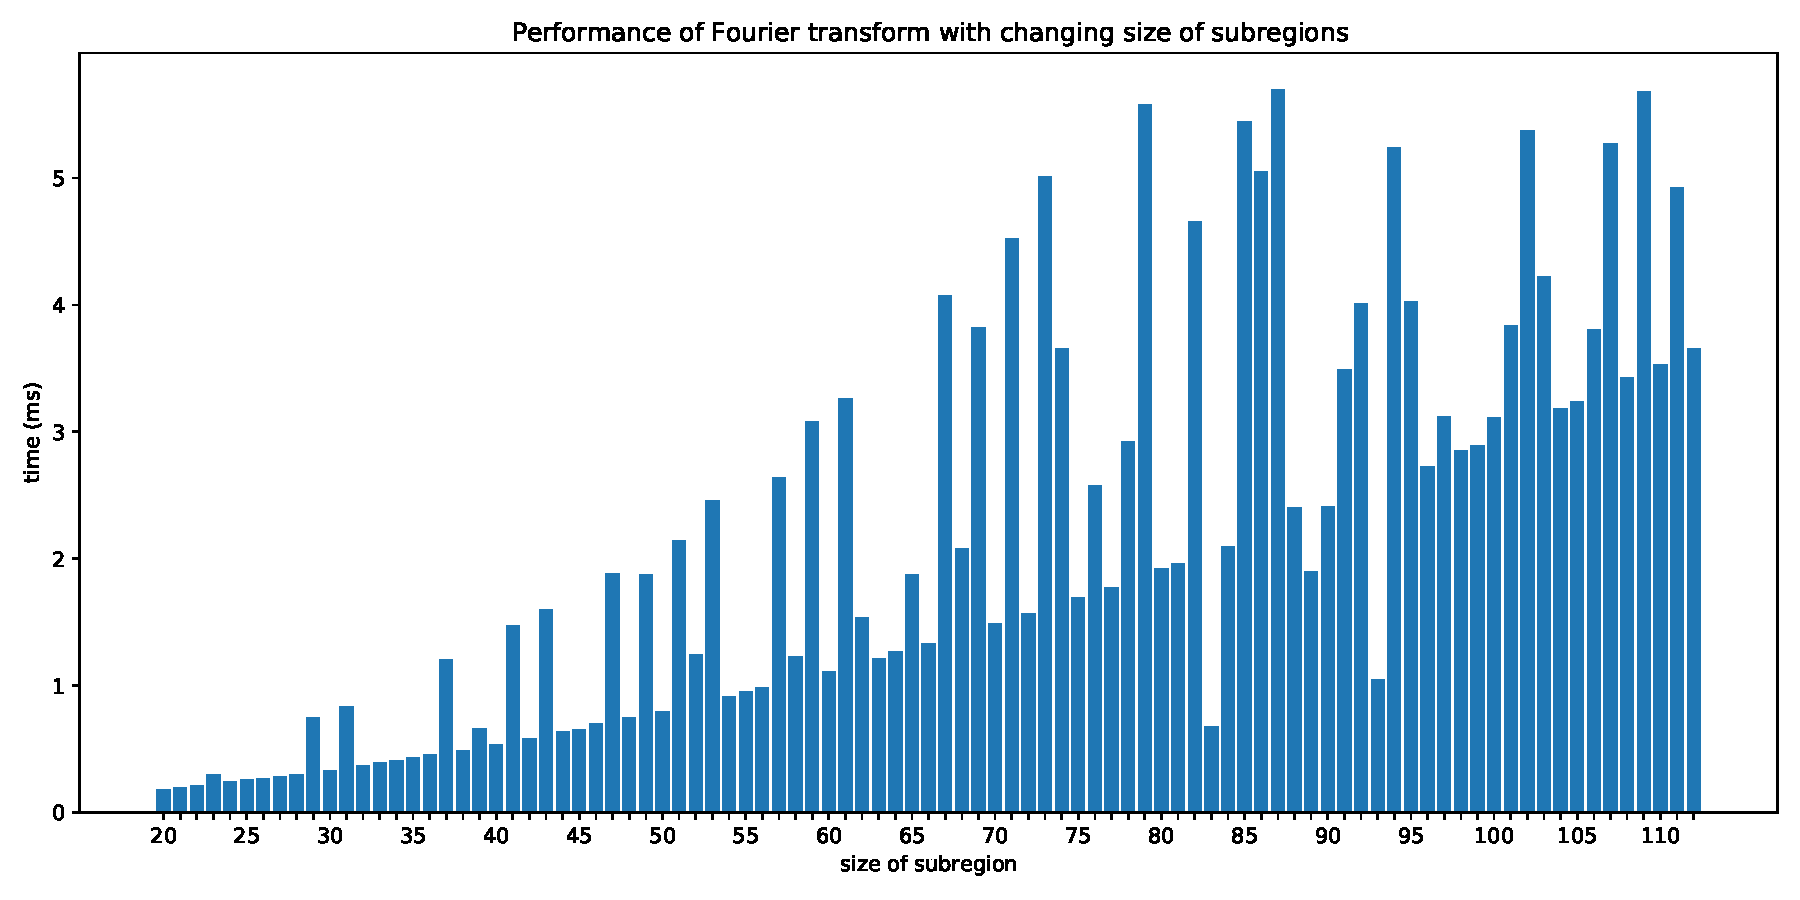
\includegraphics[width=\textwidth]{img/eval/Fourier-transform-size}
	\caption{Performance of Fourier transform with changing size of subregions. It was measured from a run of the algorithm with a configuration of 110 subregions. The size on the x axis denotes half of length of one side of subregion.}
	\label{Fourier-transform-size}
\end{figure}

In the \cref{Fourier-transform-size}, we can see how the forward Fourier transform executed by the cuFFT library depends on the size of subregions. We can see that the computation time increases with the size of the subregions, following the $\mathcal{O}(n \log n)$ time complexity of FFT, where $n$ is number of pixels. More precisely, the complexity is $\mathcal{O}(A^2 \log A)$, if $A$ denotes the length of one side of the square subregion.

However, there are quite a few outliers --- sizes, for which the function does not perform very well. That can be explained by the following sentence cited from the cuFFT documentation: ``Algorithms highly optimized for input sizes that can be written in the form $2^a3^b5^c7^d$''. It means that all sizes, whose factorization contains a prime greater than 7 perform poorly. Choosing a bigger size with nice factorization results in better performance.

We can also see, that sizes 83 and 93 perform surprisingly well. We have measured this fact consistently. The reason behind such behavior is probably specific for cuFFT implementation.

The dependence of inverse Fourier transform on size of subregions looks very similar to the \cref{Fourier-transform-size} for the same reasons.

\begin{figure}
	\begin{subfigure}{.5\textwidth}
		\centering
		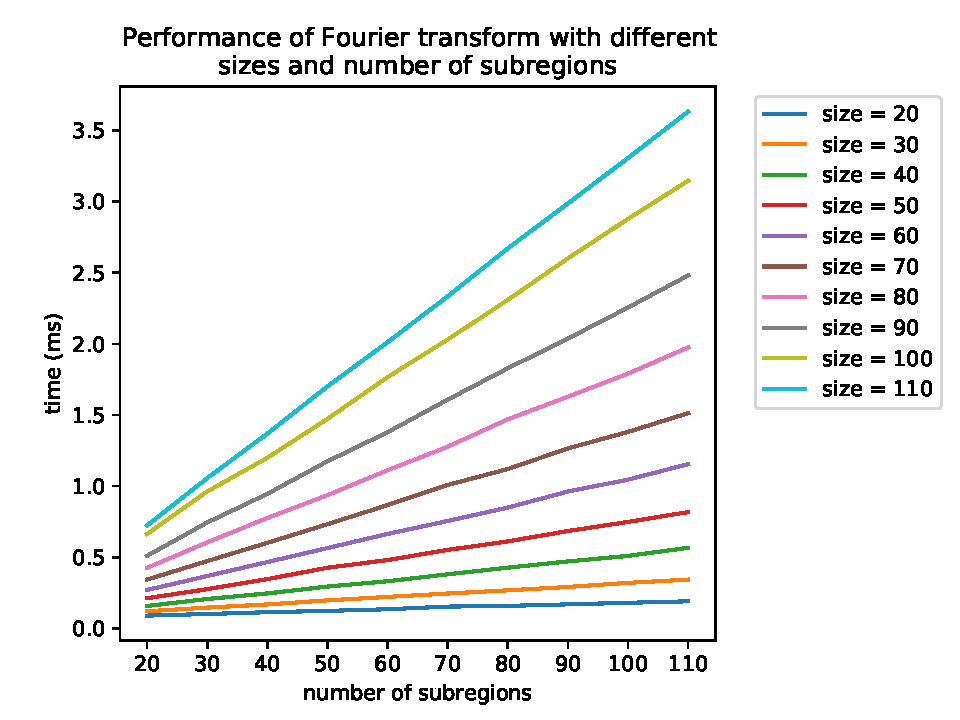
\includegraphics[width=\linewidth]{img/eval/fourier-transform-roi-count}
		\caption{}
		\label{fourier-transform-roi-count:basic}
	\end{subfigure}%
	\begin{subfigure}{.5\textwidth}
		\centering
		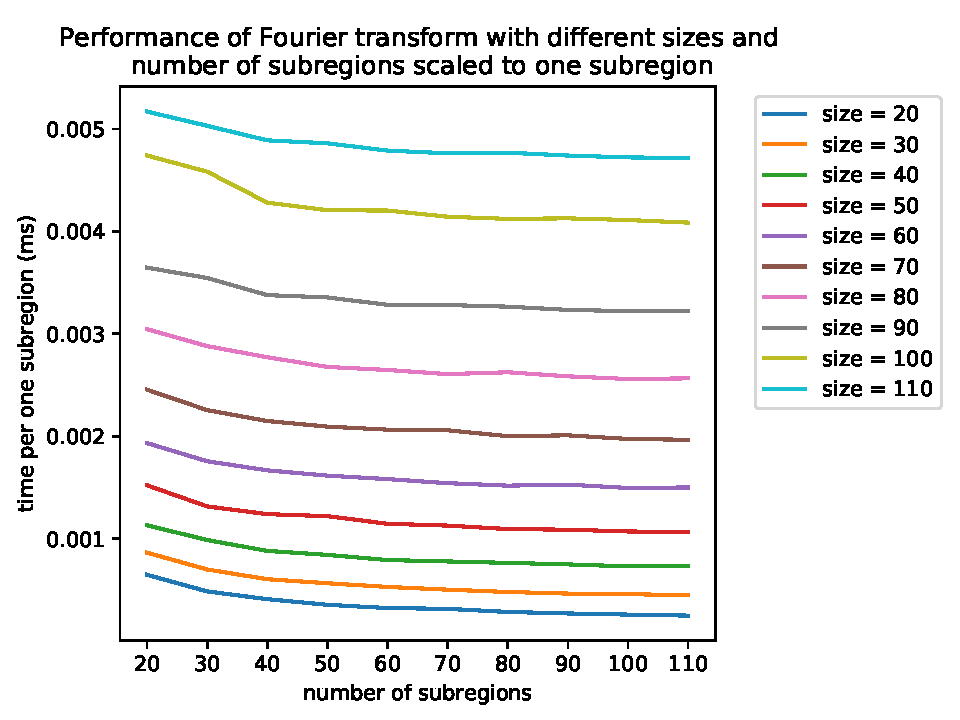
\includegraphics[width=\linewidth]{img/eval/fourier-transform-roi-count-scaled}
		\caption{}
		\label{fourier-transform-roi-count:scaled}
	\end{subfigure}
	\caption{Performance of Fourier transform with changing size and number of subregions. The size on the x axis denotes half of length of one side of subregion.}
	\label{fourier-transform-roi-count}
\end{figure}

\Cref{fourier-transform-roi-count} shows how the the Fourier transform performs with different sizes and number of subregions. \Cref {fourier-transform-roi-count:basic} shows absolute time it takes to compute the Fourier transform. As expected, the time scales roughly linearly with the number of subregions in each image.

\Cref {fourier-transform-roi-count:scaled} shows the same dependence, but the times are scaled with respect to number of subregions, so the y axis shows the average time needed to compute the Fourier transform of one subregion of respectable size. We can see that regardless of the size of subregions the library needs less time per subregion with increasing number of subregions. It is most likely caused by overhead of each CUDA kernel call --- with more subregions, the same overhead is spread over more of them, thus the computation of each subregion is cheaper. That is also the reason why we introduced the batch parameter --- to process more subregions in each run of kernel. We evaluate the impact of the batch parameter to the whole algorithm in \cref{batch-param}.

\subsection{The complex matrix multiplication}
\begin{figure}
	\begin{subfigure}{\textwidth}
		\centering
		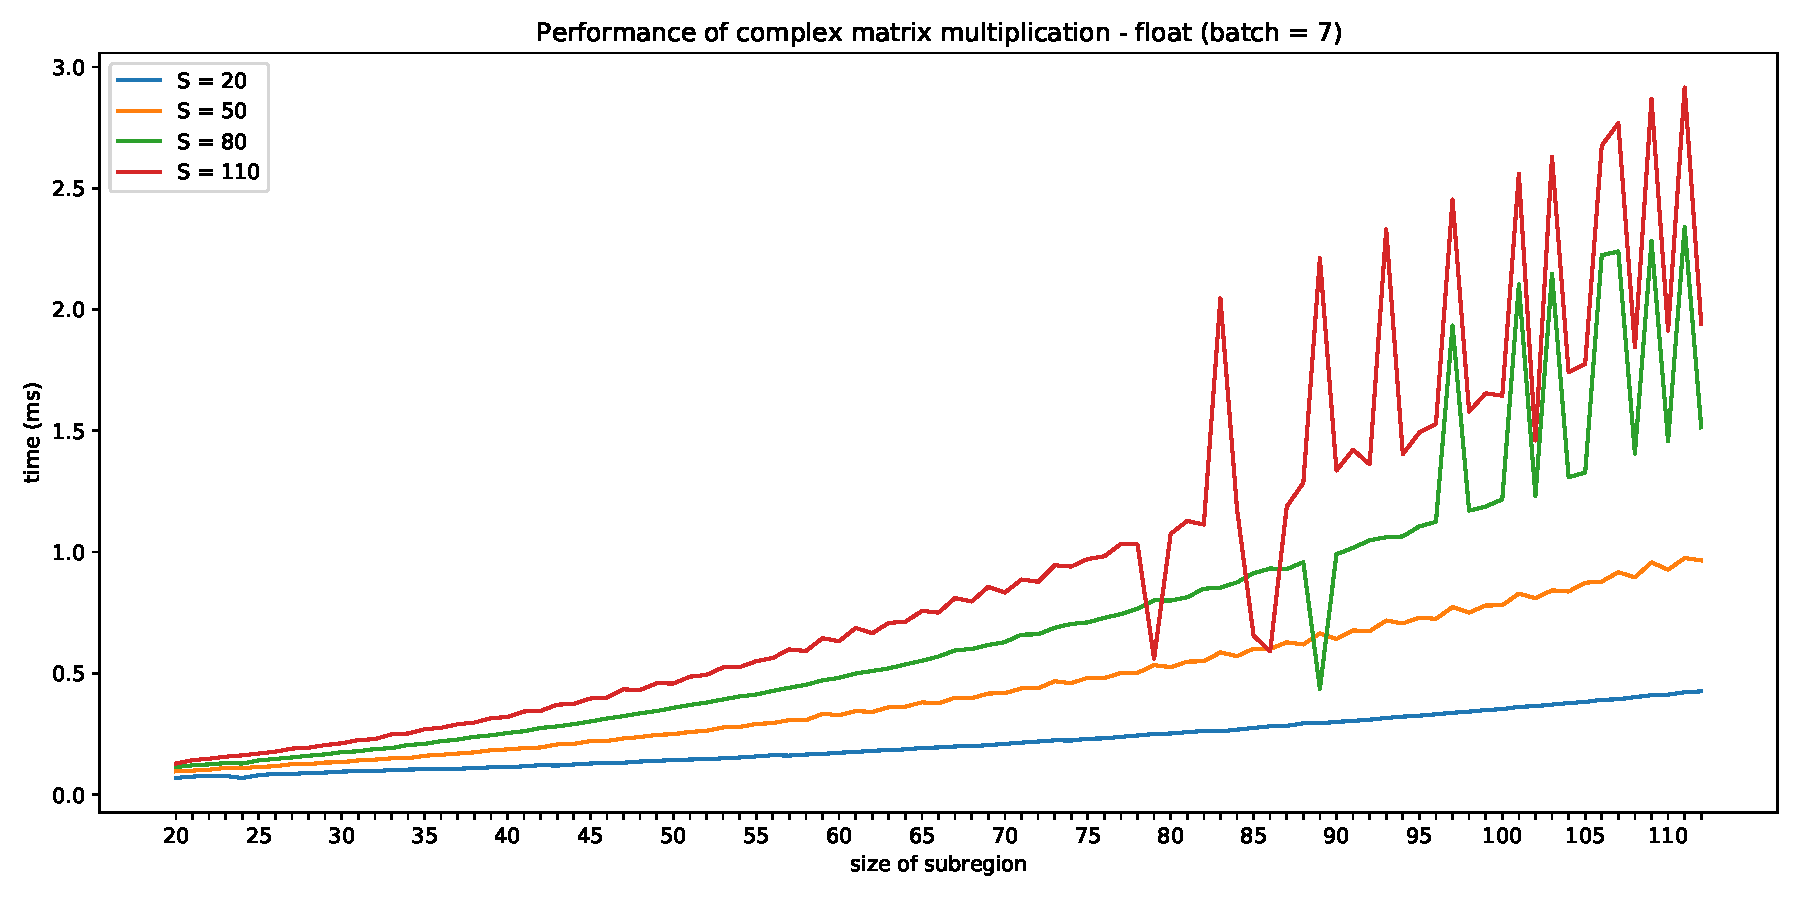
\includegraphics[width=\linewidth]{img/eval/multiply-plot-float}
		\caption{Single float precision}
		\label{multiply-plot:float}
	\end{subfigure}%

	\begin{subfigure}{\textwidth}
		\centering
		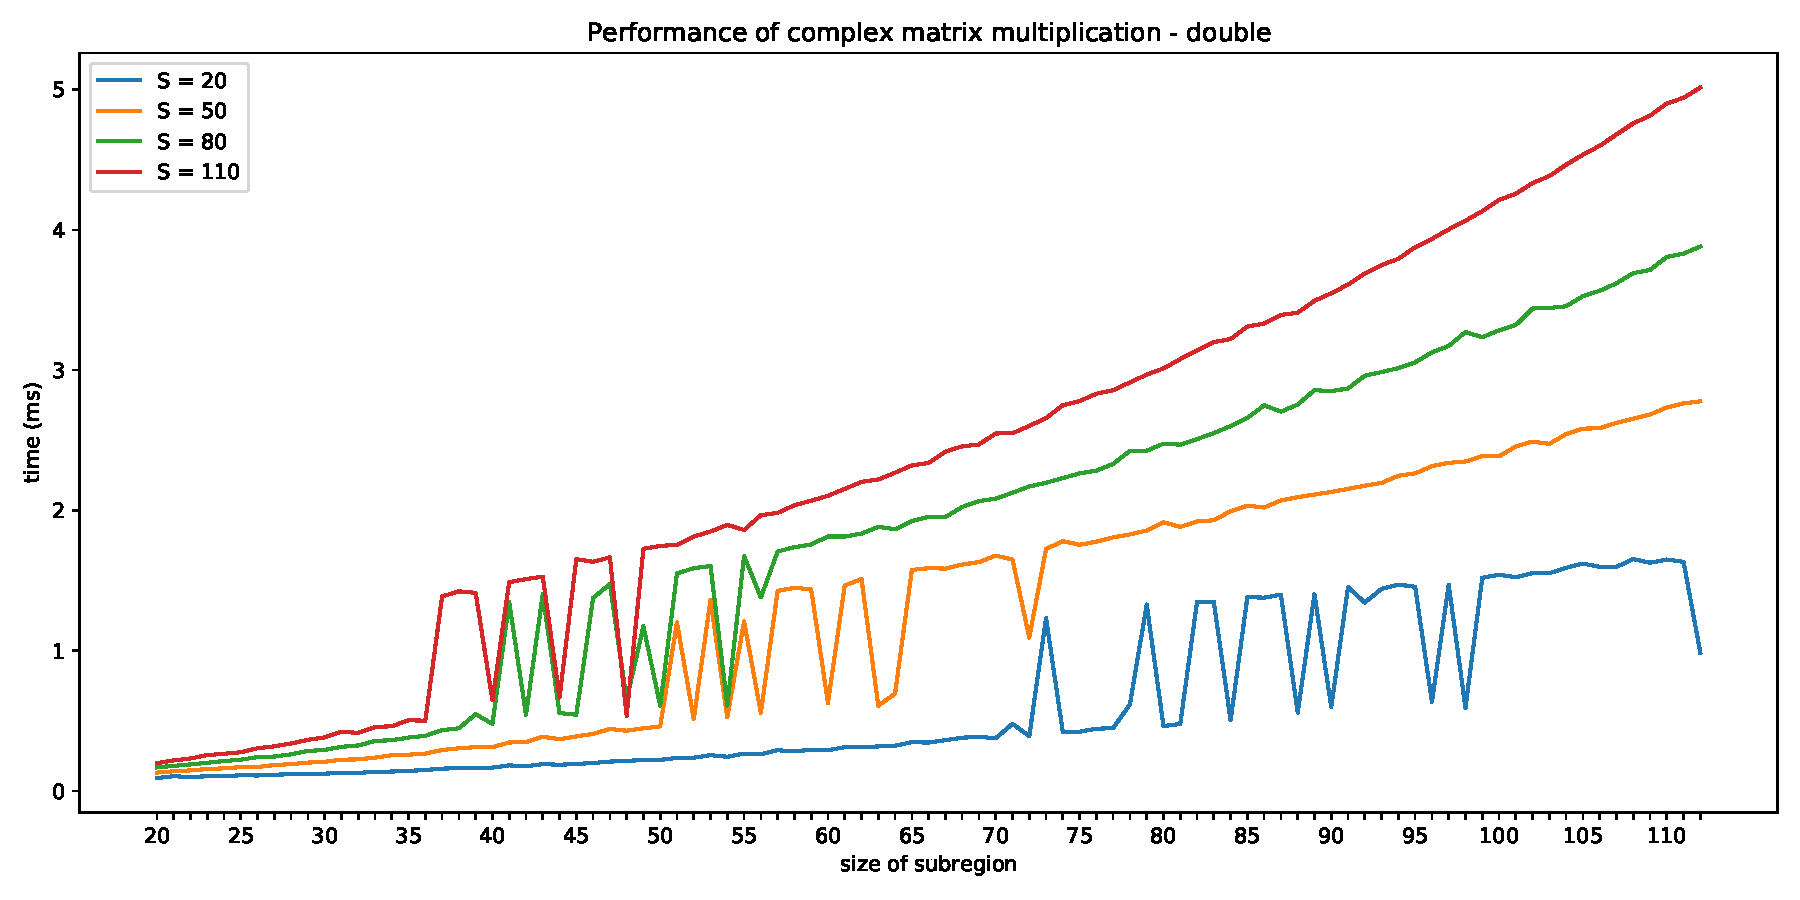
\includegraphics[width=\linewidth]{img/eval/multiply-plot-double}
		\caption{Double float precision}
		\label{multiply-plot:double}
	\end{subfigure}
	\caption{Performance of complex matrix multiplication with changing size and number of subregions. The size on the x axis denotes half of length of one side of subregion.}
	\label{multiply-plot}
\end{figure}

Another step in the cross--correlation computation is the multiplication of two complex matrices. In theory, the complexity of the multiplication is $\mathcal{O}(A^2S)$, where $A$ denotes the length of one side of the square subregion and $S$ denotes their amount. \Cref{multiply-plot} shows the measured time for different sizes and number of subregions. We can see the quadratic trend with respect to subregion size and linear with respect to their count.

However, in some cases, there seem to be a threshold over which the kernel performs worse. For float precision (\cref {multiply-plot:float}), the thresholds are higher than for double precision (\cref {multiply-plot:double}) and we do not see a consistent increase of the time for the measured sizes, only individual spikes. Unfortunately, we cannot reliably determine the relation between the threshold and algorithm parameters. It seems that the data exceed some kind of cache, but we observe worse performance for such big sizes that the processed subregions are already bigger than tens of megabytes. The plots look similar for different batch sizes too.

Moreover, we tried to measure the performance of the multiplication kernel individually and the observed worse performance was not present --- we measured clean quadratic dependency on size of subregions. That implies it is a result of some interference with the cuFFT forward Fourier transform. That would also explain the spikes, since cuFFT behaves differently for sizes with primes in their factorization. In any case, the performance difference is roughly 1ms, which is up to 10\% of total running time of whole offsets computation.

\subsection{FFT implementation versus definition--based implementation}

\begin{figure}
	\centering
	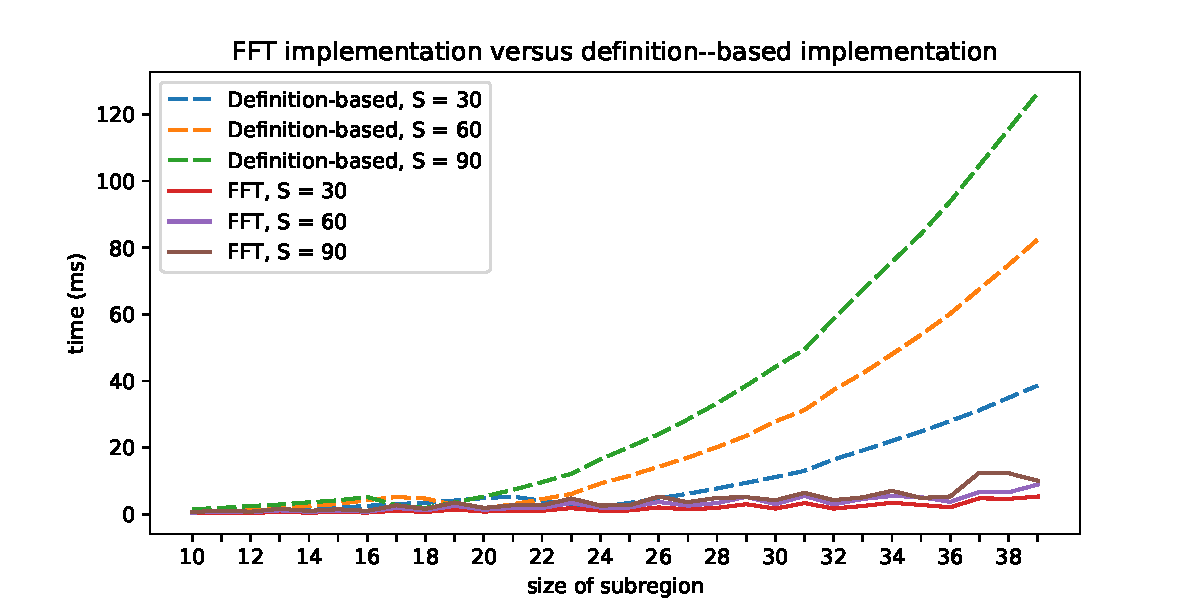
\includegraphics[width=0.8\textwidth]{img/eval/cross-compare}
	\caption{Comparison between the FFT and definition--based implementations of cross--correlation. The size on the x axis denotes half of length of one side of subregion.}
	\label{cross-compare}
\end{figure}

Recall, that we described two implementations of cross--correlation: first one based on the Fourier transform and second one based on the definition. \Cref{cross-compare} shows comparison between them --- for the FFT version, it shows the sum of average times of the Fourier transforms and complex multiplication. For the definition--based implementation, it shows the average run time of respective kernel. They are roughly the same for very small subregion sizes, but for sizes bigger than 25 the FFT implementation clearly wins. That is the minimal size of subregions that we consider useful for practical application. The conclusion is that the definition--based implementation is not useful for our application and it is always better to use the FFT implementation.


\section{Load TIFF}

\begin{figure}[h]
	\centering
	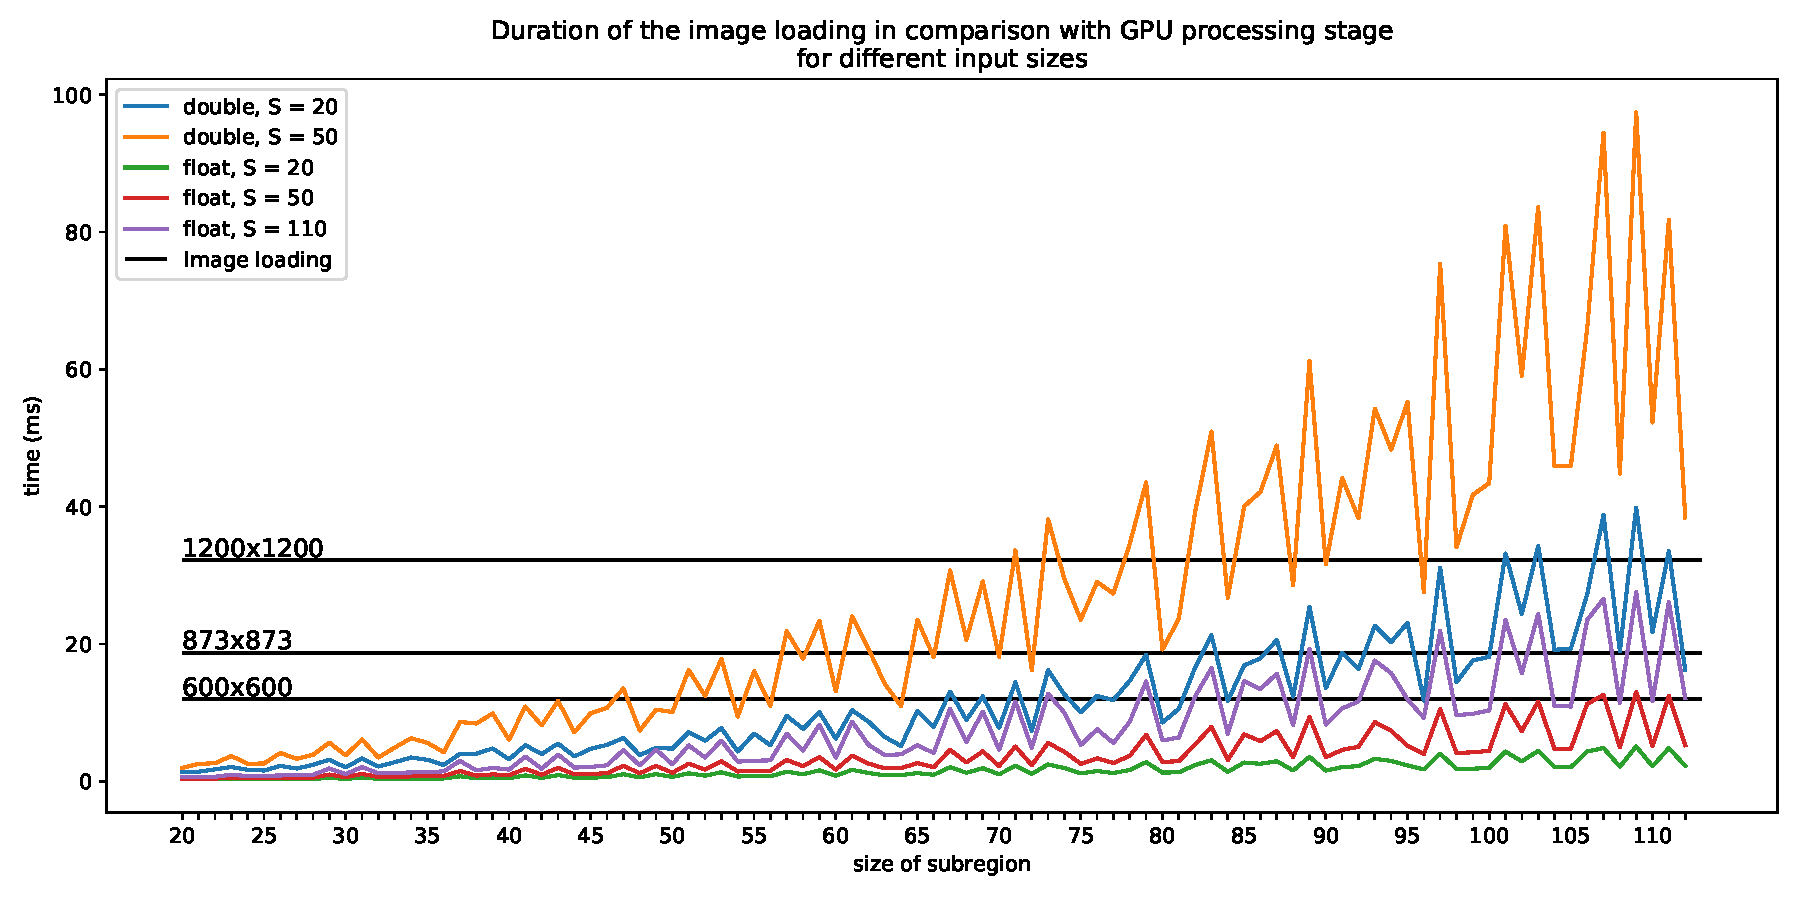
\includegraphics[width=0.8\textwidth]{img/eval/load-plot}
	\caption{}
	\label{load-wait}
\end{figure}

More workers

\section{Float versus double}


\section{Batch parameter}
\label{batch-param}


\section{Speedup compared to original python implementation}


\section{Memory consumption}


overall performance - compare with python

batch size for different subregion sizes and count

different subregion sizes and count

sum - compare N to size of one slice, to batch size, to number of slices - how?